% !TeX root = Trafficsimulation_Documentation.tex

\chapter{Software-Architektur}
\label{Software-Architektur}

In diesem Kapitel werden im ersten Schritt die Komponenten der Software grafisch, in Form von Deployment- und Komponenten-Diagrammen, beschrieben. Darauf folgt im Abschnitt \ref{Textuelle Beschreibung} eine textuelle Beschreibung der zuvor grafisch visualisierten Komponenten, deren Zusammenhänge und Funktionalitäten.

\thispagestyle{standard}
\pagestyle{standard}

\section{Grafische Beschreibung}
\label{Grafische Beschreibung}

\begin{figure}[H]
\begin{center}
	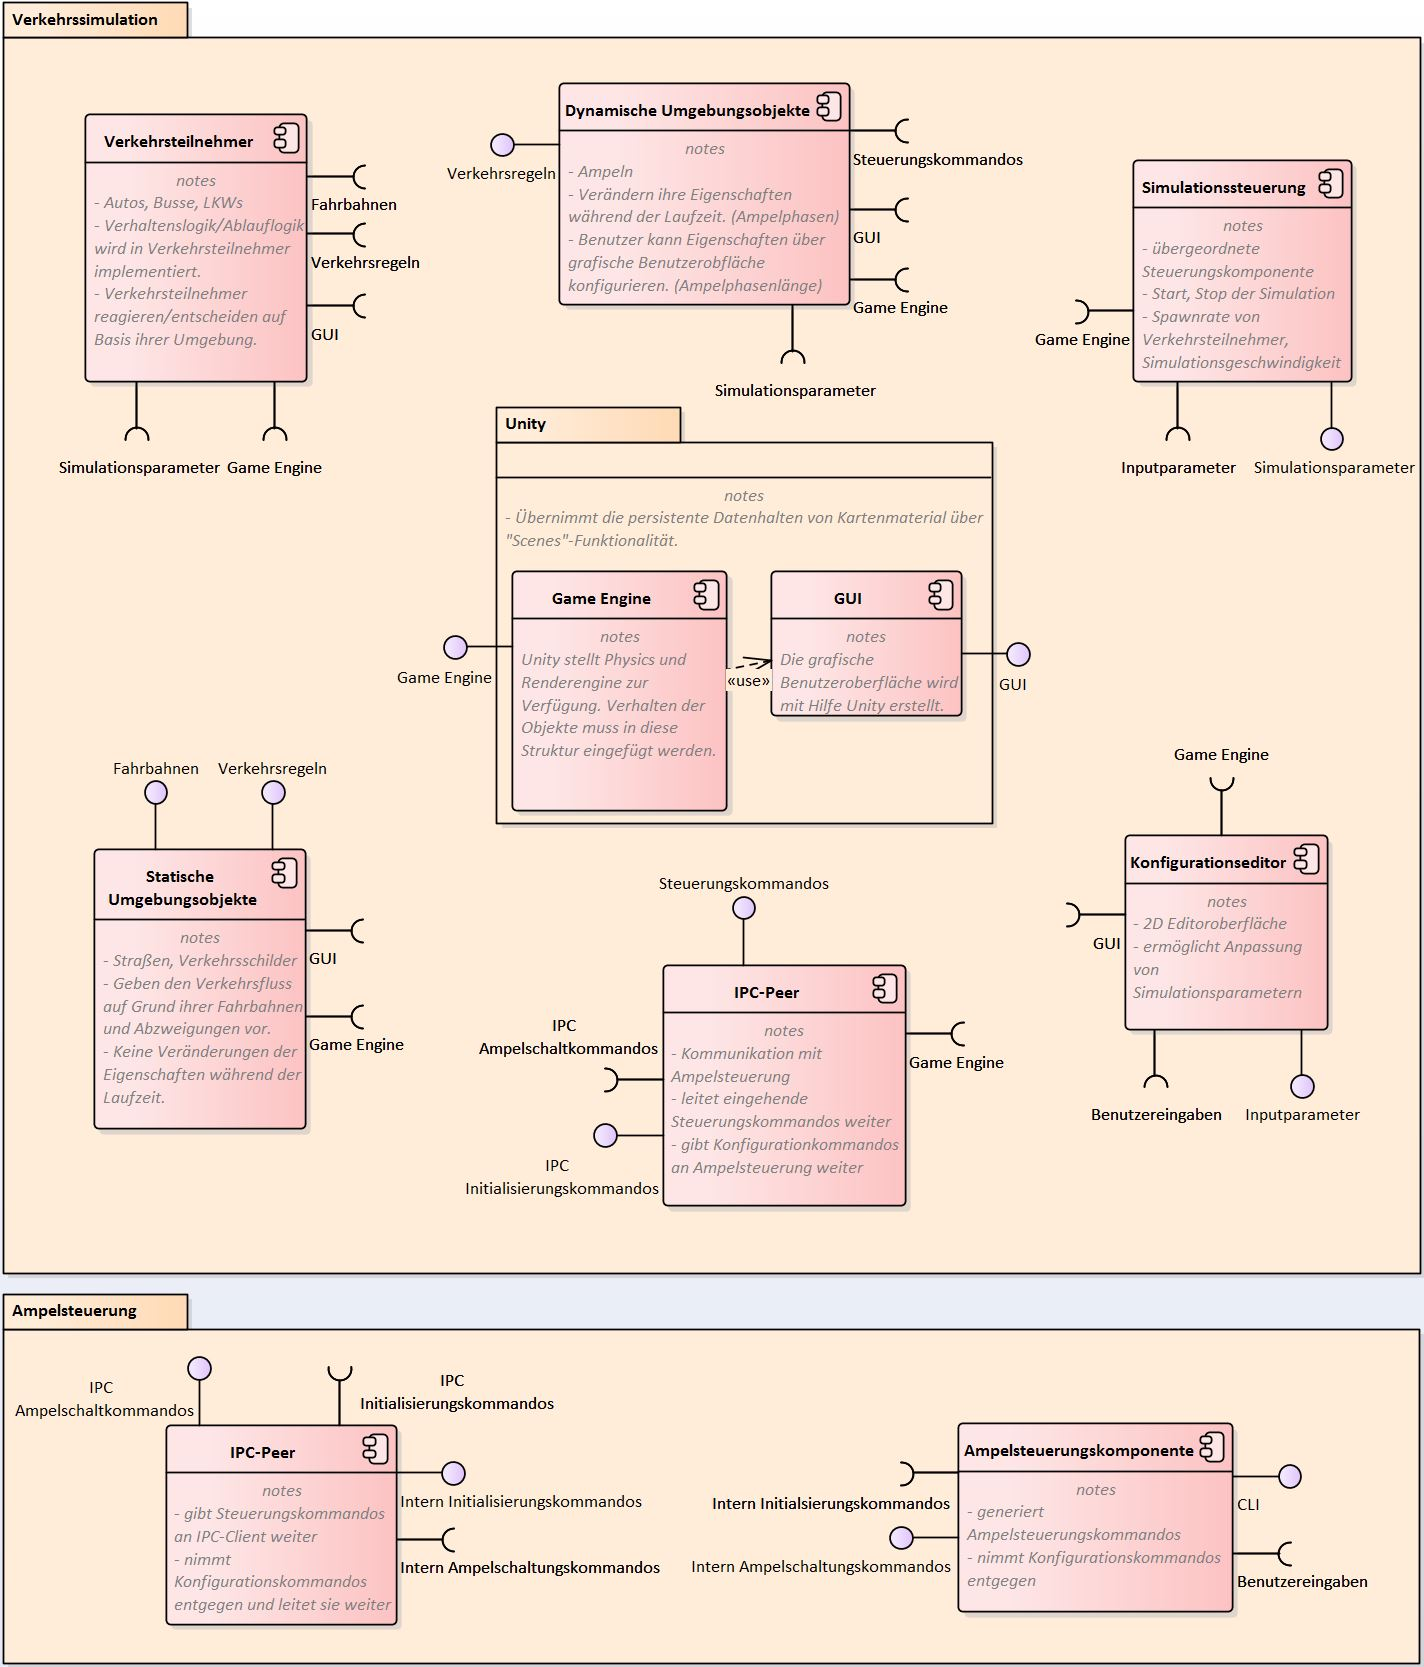
\includegraphics[scale=0.673]{BilderAllgemein/Komponentdiagram.JPG}
\end{center}
	%\includegraphics[width=\textwidth]
	%\end{center}
	% Title
	\caption{Komponenten Diagramm Verkehrssimulation}
	% Unique name: identifier for referencing
	%\label{Abbildung 2.1}
\end{figure}

\section{Textuelle Beschreibung}
\label{Textuelle Beschreibung}

In diesem Abschnitt folgt die textuelle Beschreibung der unter Punkt \ref{Grafische Beschreibung} angeführten Komponenten.

\begin{flushleft}
\textbf{Verkehrssimulation und Ampelsteuerung}
\end{flushleft}
\vspace{-0.3 cm}

Sowohl Verkehrssimulation als auch Ampelsteuerung sind eigene Executables. Die Verkehrssimulation wird aus dem Unity-Projekt erzeugt und beinhaltet alle oben angegebenen Komponenten. Die Ampelsteuerung ist eine Konsolen Applikation, welche über die IPC-Komponenten mit der Verkehrssimulation kommuniziert.

\begin{flushleft}
\textbf{Verkehrsteilnehmer}
\end{flushleft}
\vspace{-0.3 cm}

Zu diesen Komponenten gehören alle sich aktiv in der Simulation bewegenden Objekte, wie Autos, Busse und LKWs. Die einzelnen Komponenten bewegen sich autonom voneinander im Straßennetz fort. Die Komponenten scannen ihre Umgebung auf Fahrbahnen, Verkehrsregeln und andere Verkehrsteilnehmer. Auf Basis dieses Scans entscheiden sie ihre nächste Aktion, wie zum Beispiel Beschleunigen, Bremsen oder Abbiegen. Verkehrsteilnehmer können sich ausschließlich auf Fahrbahnen bewegen und beachten alle Verkehrsregeln innerhalb ihres Aktionsradius. Weiters benötigen sie Simulationsparameter, die über ihre maximale Geschwindigkeit, Beschleunigung und Bremsverhalten entscheiden. Verkehrsteilnehmer treffen ihre Entscheidungen bei jedem Renderdurchlauf der Game Engine. Die Verknüpfung der Verkehrsteilnehmer mit der GUI erfolgt abstrahiert durch Unity.

\begin{flushleft}
\textbf{Dynamische Umgebungsobjekte}
\end{flushleft}
\vspace{-0.3 cm}

Dynamische Umgebungsobjekte sind Objekte, welche während der Simulationslaufzeit ihre Eigenschaften ändern, jedoch nicht ihre Position. Konkret sind dynamische Umgebungsobjekte Ampeln. Ampeln bieten den umliegenden Verkehrsteilnehmern ihren derzeitigen Status als Verkehrsregeln an, welche diese beachten müssen. Dynamische Elemente benötigen Simulationsparameter, welche ihre Schaltzeiten vorgeben. Konkret geben die Simulationsparameter die Phasenzeiten der Ampeln an. Weiters benötigen dynamische Umgebungsobjekte Steuerungskommandos um zwischen diversen Modi zu wechseln. Über Steuerungskommandos können Ampeln von automatischen Betrieb in einen inaktiven dauerhaft Gelb blinkenden Status gebracht werden. In jedem Renderzyklus der Game Engine wird auf neue Steuerungskommandos geprüft und falls nötig der vorgegebene Schaltvorgang eingeleitet. Die Verknüpfung der dynamischen Umgebungsobjekte mit der GUI erfolgt abstrahiert durch Unity.

\begin{flushleft}
\textbf{Simulationssteuerung}
\end{flushleft}
\vspace{-0.3 cm}

Die Simulationssteuerung stellt eine übergeordnete Kontrollinstanz der Simulation dar. Sie legt globale Einstellungen für Simulationskomponenten zentral fest. Die Simulationssteuerung bietet Simulationsparameter für andere Simulationskomponenten an, welche diese abrufen können. Konkrete Simulationsparameter sind Schaltzeiten für Ampeln, Höchstgeschwindigkeiten für Verkehrsteilnehmer oder Spawnraten für neue Verkehrsteilnehmer. Die Simulationssteuerung benötigt Inputparameter, welche von außen die Simulationsparameter bestimmen. Die Aktualisierung der Simulationsparameter auf Basis der Inputparameter erfolgt bei jedem Renderzyklus der Game Engine.

\begin{flushleft}
\textbf{Konfigurationseditor}
\end{flushleft}
\vspace{-0.3 cm}

Der Konfigurationseditor stellt eine zweidimensionale graphische Benutzeroberfläche dar, welche es dem Benutzer ermöglicht angebotene Inputparameter für die Simulation zu verändern. Vom Benutzer geänderte Inputparameter werden bei jedem Renderzyklus der Game Engine verarbeitet und entsprechend weiter geleitet.

\begin{flushleft}
\textbf{IPC-Peer Verkehrssimulation}
\end{flushleft}
\vspace{-0.3 cm}

Der IPC-Peer Verkehrssimulation repräsentiert eine Instanz der Inter Process Communication zwischen den Executables Verkehrssimulation und Ampelsteuerung dar. Dieser IPC-Peer gibt Initialisierungskommandos an die Ampelsteuerung weiter. Über diese Kommandos werden die benötigte Anzahl an Ampeln mit den korrekten Initialisierungsparametern angelegt. Weiters werden Ampelschaltkommandos entgegen genommen und weiter geleitet um den Modus einer Ampel zu wechseln. Ein- und ausgehende Kommandos während in jedem Renderzyklus der Game Engine bearbeitet.

\begin{flushleft}
\textbf{Statische Umgebungsobjekte}
\end{flushleft}
\vspace{-0.3 cm}

Statische Umgebungsobjekte repräsentieren Simulationskomponente, welche weder ihre Eigenschaften noch ihre Position während der Simulationslaufzeit verändern. Konkret sind Straßen und Verkehrsschilder statische Umgebungsobjekte. Sie bieten Fahrbahnen für die Verkehrsteilnehmer an, auf welchen diese sich bewegen können. Zusätzlich werden auch Verkehrsregeln vorgegeben, welche von den Verkehrsteilnehmer beachtet werden müssen. Die statischen Umgebungsobjekte werden von der Game Engine gerendert, jedoch sollte diese Komponente keine Logik besitzen. Die Verknüpfung der statischen Umgebungsobjekte mit der GUI erfolgt abstrahiert durch Unity.

\begin{flushleft}
\textbf{IPC-Peer Ampelsteuerung}
\end{flushleft}
\vspace{-0.3 cm}

Die Komponente IPC-Peer Ampelsteuerung bildet die Gegenstelle der zuvor beschriebenen IPC-Peer Verkehrssimulation. Sie gibt Ampelschaltkommandos zur Gegenstelle weiter und nimmt Initialisierungskommandos entgegen. Diese Kommandos werden intern, innerhalb der Ampelsteuerung Executable an die Ampelsteuerungskomponente weiter gegeben.

\begin{flushleft}
\textbf{Ampelsteuerungskomponente}
\end{flushleft}
\vspace{-0.3 cm}

Die Ampelsteuerungskomponente übernimmt die Verwaltung der einzelnen Ampelinstanzen. Anhand eingehender Initialisierungskommandos werden Ampelinstanzen mit den benötigten Initialisierungsparametern erstellt. Über das angebotene CLI kann der Benutzer Schaltbefehle absetzen, welche über Ampelschaltungskommandos weiter geleitet werden.




\begin{flushleft}
\textbf{Message Queue}
\end{flushleft}
\vspace{-0.3 cm}

Die Message Queue übernimmt die Kommunikation mit den anderen Gruppen. Die Kommunikation mit den anderen Gruppen wird über einen externen Server abgewickelt, auf denen sich die Gruppen anmelden und ihre Queues abonnieren können. Ein Format, basierend auf JSON wurde zwischen den Gruppenteilnehmern definiert.

Als Protokoll wird dabei AMPQ verwendet, der dazugehörende Server, RabbitMQ implementiert diese Protokoll und ermöglicht die Übertragung von Nachrichten.
